\documentclass[CS5104-Notes.tex]{subfiles}
\begin{document}

\section{Regularisation}
When using too many features, it is often the case that overfitting happens where the model fits well to the training data, but does not generalise to unseen data. A typical way to deal with overfitting is to reduce the number of features, either manually or automatically. This is done because some input features may not be very relevant to the general problem, but still affect the prediction. 
\n
\textbf{Regularisation} is another method to reduce the effect of some input features without removing them completely. It works by keeping all input features, but using multipliers to reduce the scale of certain $\theta$ parameters. This allows more relevant features to have more impact while still keeping a lower effect of less relevant features. The parameters are penalised using a large multiplier to cause them to be minimised because of the increased constant. For example $... + 1000\theta_{3} + 1000\theta_{4}$. This changes the cost function by adding a regularisation parameter $\lambda$.
\begin{equation}
\text{Cost} = \frac{1}{2m}\bigg[\sum_{i=0}^{m}(h(x^{i}) - y^{i})^{2} + \lambda \sum_{j=1}^{n}\theta_{j} \bigg]
\end{equation}
The regularisation parameter $\lambda$ determines how much to suppress the $\theta$ parameters. If $\lambda$ is too large, then we may underfit as we have minimised the $\theta$ parameters too much. If $\lambda$ is too small, then we may continue to overfit as it does not do enough to reduce the effect of $\theta$ parameters. 
\n
The regularisation parameter can also be added to the normal equation.
\begin{equation}
\theta = \Bigg( X^{T}X + \lambda \begin{bmatrix} 
	0 & 0 & 0 & 0 \\
	0 & 1 & 0 & 0 \\
	0 & 0 & 1 & 0 \\
	0 & 0 & 0 & 1
\end{bmatrix}  \Bigg)^{-1}X^{T}y
\end{equation}
In general, regularisation can be thought of as adding an extra component to the equation of minimising the cost function.
\begin{equation}
J(\theta) = L(\theta) + R(\theta)
\end{equation}
where $J(\theta$ is the cost, $L(\theta)$ is the loss and $R(\theta)$ is the regularisation. Further, regularisation has a computational advantage over feature selection, as additional training and searching of models is not needed.
\subsection{Ridge regression}
The $\lambda \sum_{j=1}^{n}\theta_{j}$ term for regularisation can be calculated using the $l_{2}$ norm, usually denoted as $||\theta||_{2}^{2}$. The $l_{2}$ norm is the euclidean norm, which is a sum of squares of all elements, defined as:
\begin{equation}
||\theta||_{2} = \sqrt{\sum_{j=1}^{n}\theta_{j}^2}
\end{equation}
It measures the distance of $\theta$ from zero. As $\lambda$ increases, the $l_{2}$ norm will \textit{always} decrease. The reason regularisation has an advantage of a simple least squares regression is based on the \textbf{bias-variance trade-off}. As $\lambda$ increases, the flexibility of the model decreases, leading to decreased variance, but increased bias. For some values of $\lambda$ up to a limit, the variance will decrease rapidly with only a small increase in bias, which reduces the overall mean squared error of the model. 
\begin{figure}[H]
\centering
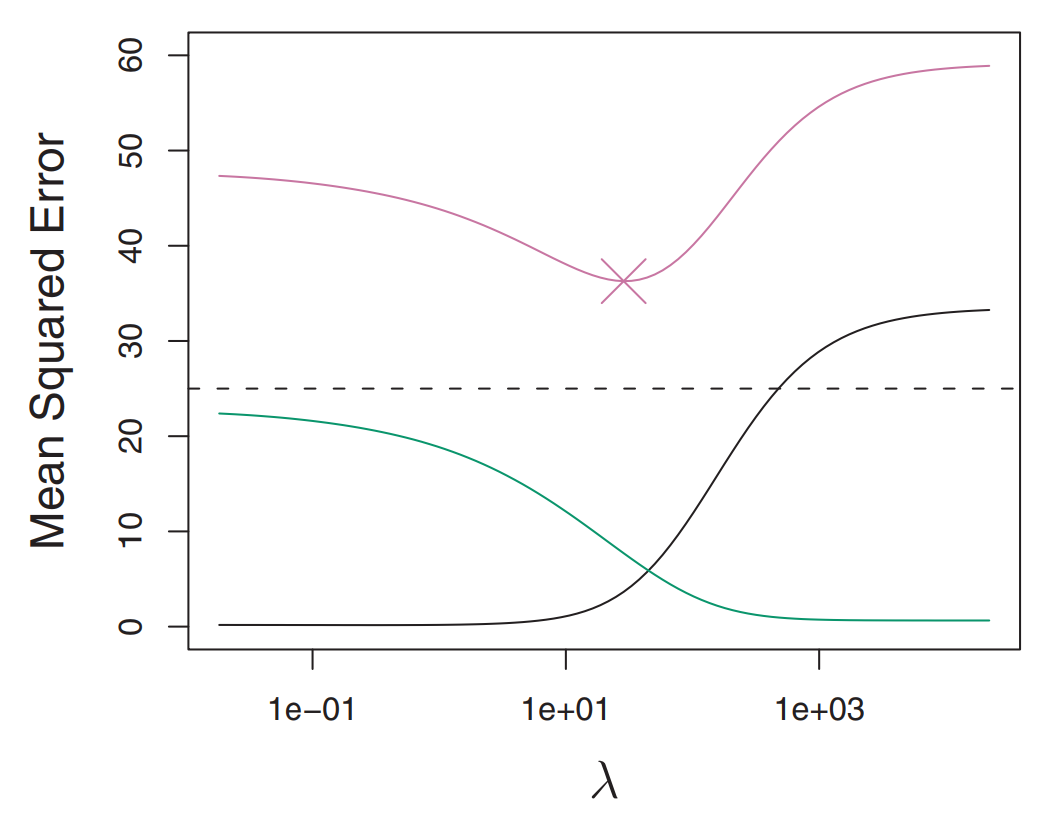
\includegraphics[width=0.6\textwidth, keepaspectratio]{imgs/ridge-regression.png}
\caption{Plot showing why ridge regression leads to lower MSE for some values of $\lambda$. Squared bias (black), variance (green) and test MSE (purple) for the ridge regression predictions on a simulated dataset as a function of $\lambda$. Taken from \textit{An Introduction to Statistical Learning}.}
\end{figure}
\subsection{Lasso regression}
The disadvantage of ridge regression is that while it will shrink all coefficients towards zero, it will not set them to be exactly zero unless $\lambda = \infty$. In other words, for datasets with a large number of features, increasing $lambda$ will reduce their effect but not exclude any of them completely.
\n
Lasso regression works the same way as ridge regression, except instead of using the $l_{2}$ norm, the $l_{1}$ norm is used. Rather than being a sum of squares, the $l_{1}$ norm is simply a sum of all elements.
\begin{equation}
||\theta||_{1} = \sum_{j=1}^{n}|\theta_{j}|
\end{equation}
Lasso regression also shrinks the coefficient estimates towards zero. However, the $l_{1}$ penalty is able to force some coefficient estimates to be equal to zero when the $lambda$ value is large enough. In this sense, lasso regression performs variable selection like selecting the best features. It can be said that lasso regression yields \textit{sparse} models because the models may only involve a smaller subset of features. 
\section{Evaluation}
The goal of supervised machine learning is to train the models on known data in order to predict new data. To be able to evaluate how well the model works on new data, any given data has to be split into separate training and test data sets. The testing data is used as a final step after training models to evaluate how well they perform. Testing data should \textit{never} be used to train, as otherwise this would bias the model heavily towards the testing data, rather than towards general unseen data. Further, testing data should not be used for any step of the machine learning process except for checking the performance of trained models at the very end. 
\subsection{Source of errors}
\begin{itemize}
\item Not enough data which leads to overfitting to available data and inability to generalise
\item Fine tuning parameters on test data which still causes overfitting because the model is designed to work well only on available data
\item Training or making decisions based on testing data could lead to very low error rates on available data, but the heavy bias is undesirable
\end{itemize}
Most often, the source of errors in machine learning comes from overfitting in some way, either from looking and training towards the test data, or from not enough data or too many input features.

\subsection{Classification metrics}
Classification differs from regression in that all errors are treated the same. It is not as easy as using functions such as the root mean squared error or $R^{2}$ coefficient of determination. Classification are either correct or incorrect, which makes errors simpler as there is no need to calculate how far the predicted value is.
\begin{itemize}
\item Correct classification = true positives + true negatives
\item Incorrect classification = false positives + false negatives
\end{itemize}

\begin{figure}[H]
\centering
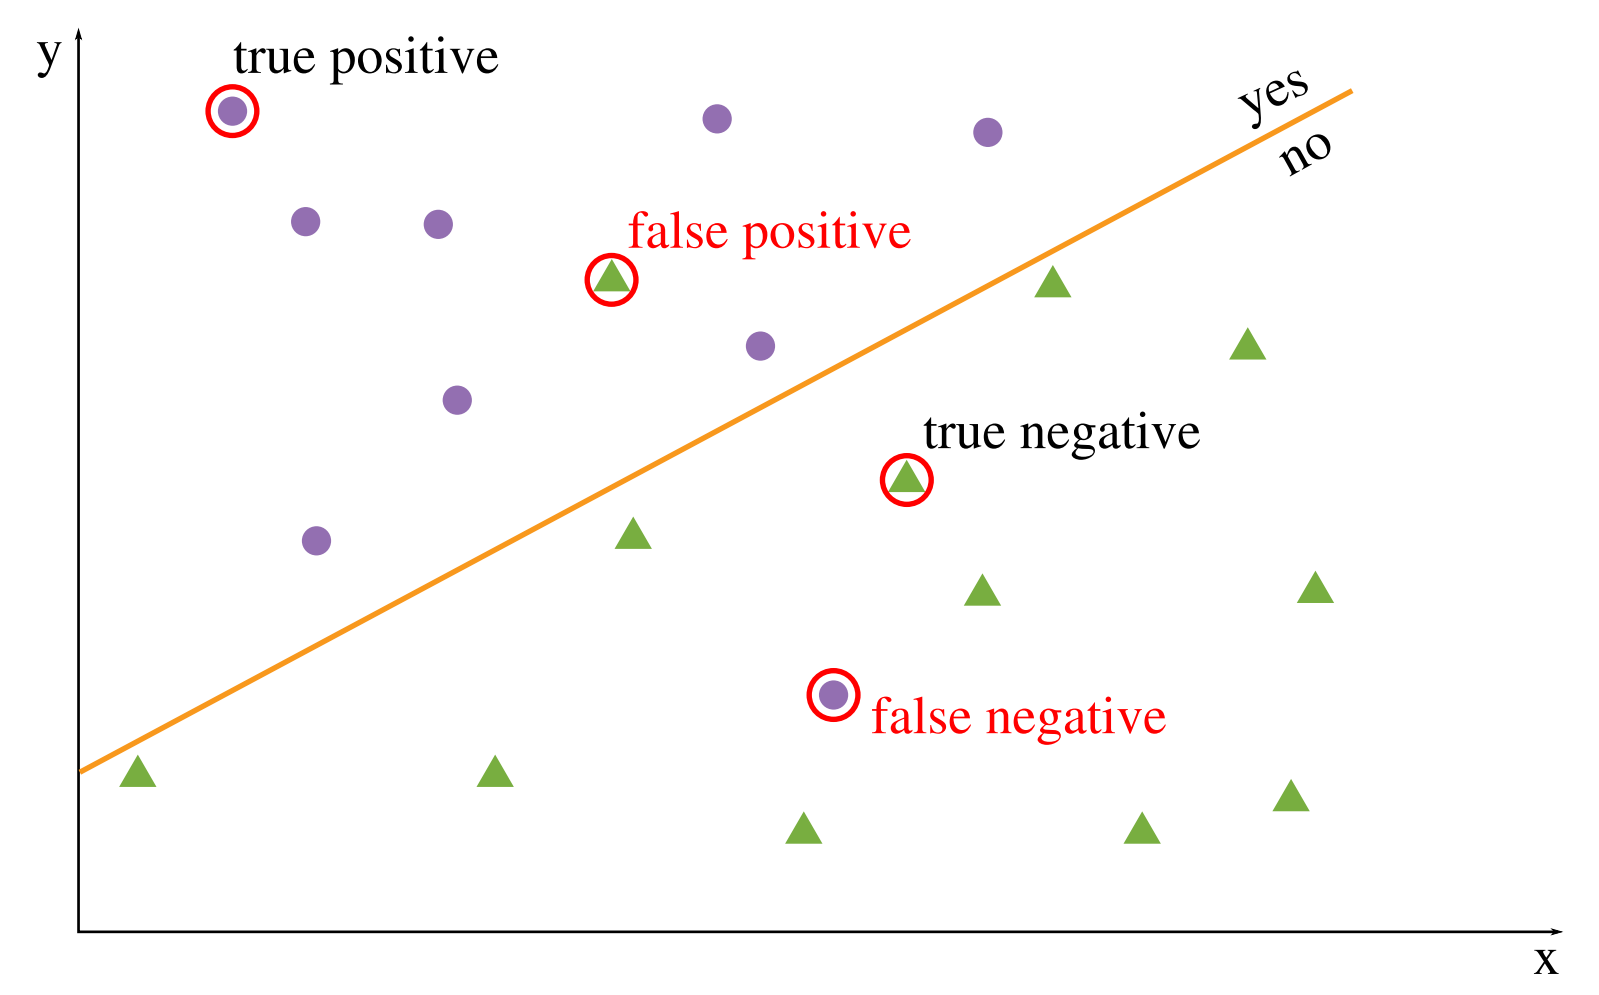
\includegraphics[width=0.9\textwidth, keepaspectratio]{imgs/classification-metrics.png}
\caption{Examples of the different types of correct/incorrect classification}
\end{figure}
\noindent
With different combinations of true/false positives/negatives, different metrics can be calculated for classification problems. For example, the accuracy (or classification rate) is defined as:
\begin{equation}
\text{accuracy} = \frac{\text{true positives} + \text{true negatives}}{\text{total positives} + \text{total negatives}}
\end{equation}
There are many further metrics that can be used for classification, most notably are \textbf{precision} and \textbf{recall}.
\begin{align}
\text{precision} &= \frac{\text{true positives}}{\text{true positives} + \text{false positives}} \\
\text{recall} &= \frac{\text{true positives}}{\text{true positives} + \text{false negatives}}
\end{align}
The precision is the fraction of correct classifications among all classified data points and the recall is the fraction of correct classifications among all relevant data points. In other words, the precision tells us how much of what was classified is correctly classified, while the recall tells us how much of the positive classifications were found out of the total positive data points. The two scores represent a trade-off as to how correct the classifications are against how many relevant data points were found. This trade-off depends on the actual classification problem. For example, in the case of cancer identification, it may be better to bias towards false positives (higher recall, lower precision) to be on the safe side.
\n
The trade-off between precision and recall can often be visualised by varying a threshold on the classification and plotting a precision-recall curve. 
\begin{figure}[H]
\centering
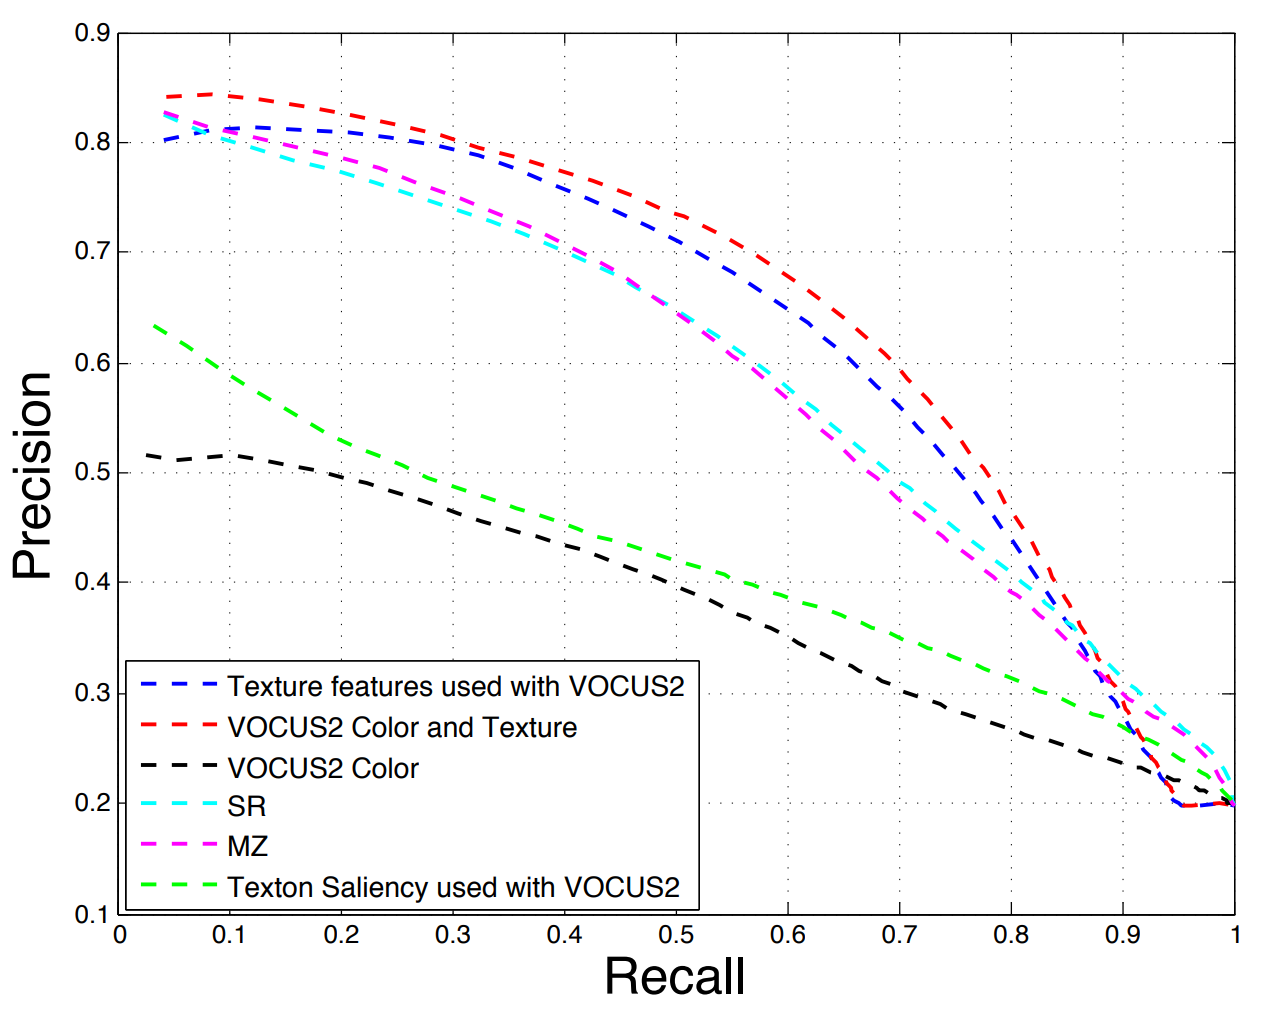
\includegraphics[width=0.6\textwidth, keepaspectratio]{imgs/precision-recall.png}
\caption{Precision-recall curves.}
\end{figure}
\noindent
It is often difficult to compare precision-recall curves as different curves could represent different trade-offs. It is more useful to have a single number to compare, so the area under the curve is used as an alternative. The larger the area, the better the performance. This is because a good model that achieves both high precision and recall will have a larger area under the curve. This area is the \textbf{average precision} for one binary classification task averaged over all possible parameter values. With multiple classes, a precision-recall curve would be needed for each class in the one-vs-all method. To better visualise this for an average over all classes, a \textbf{confusion matrix} can be used.
\begin{figure}[H]
\centering
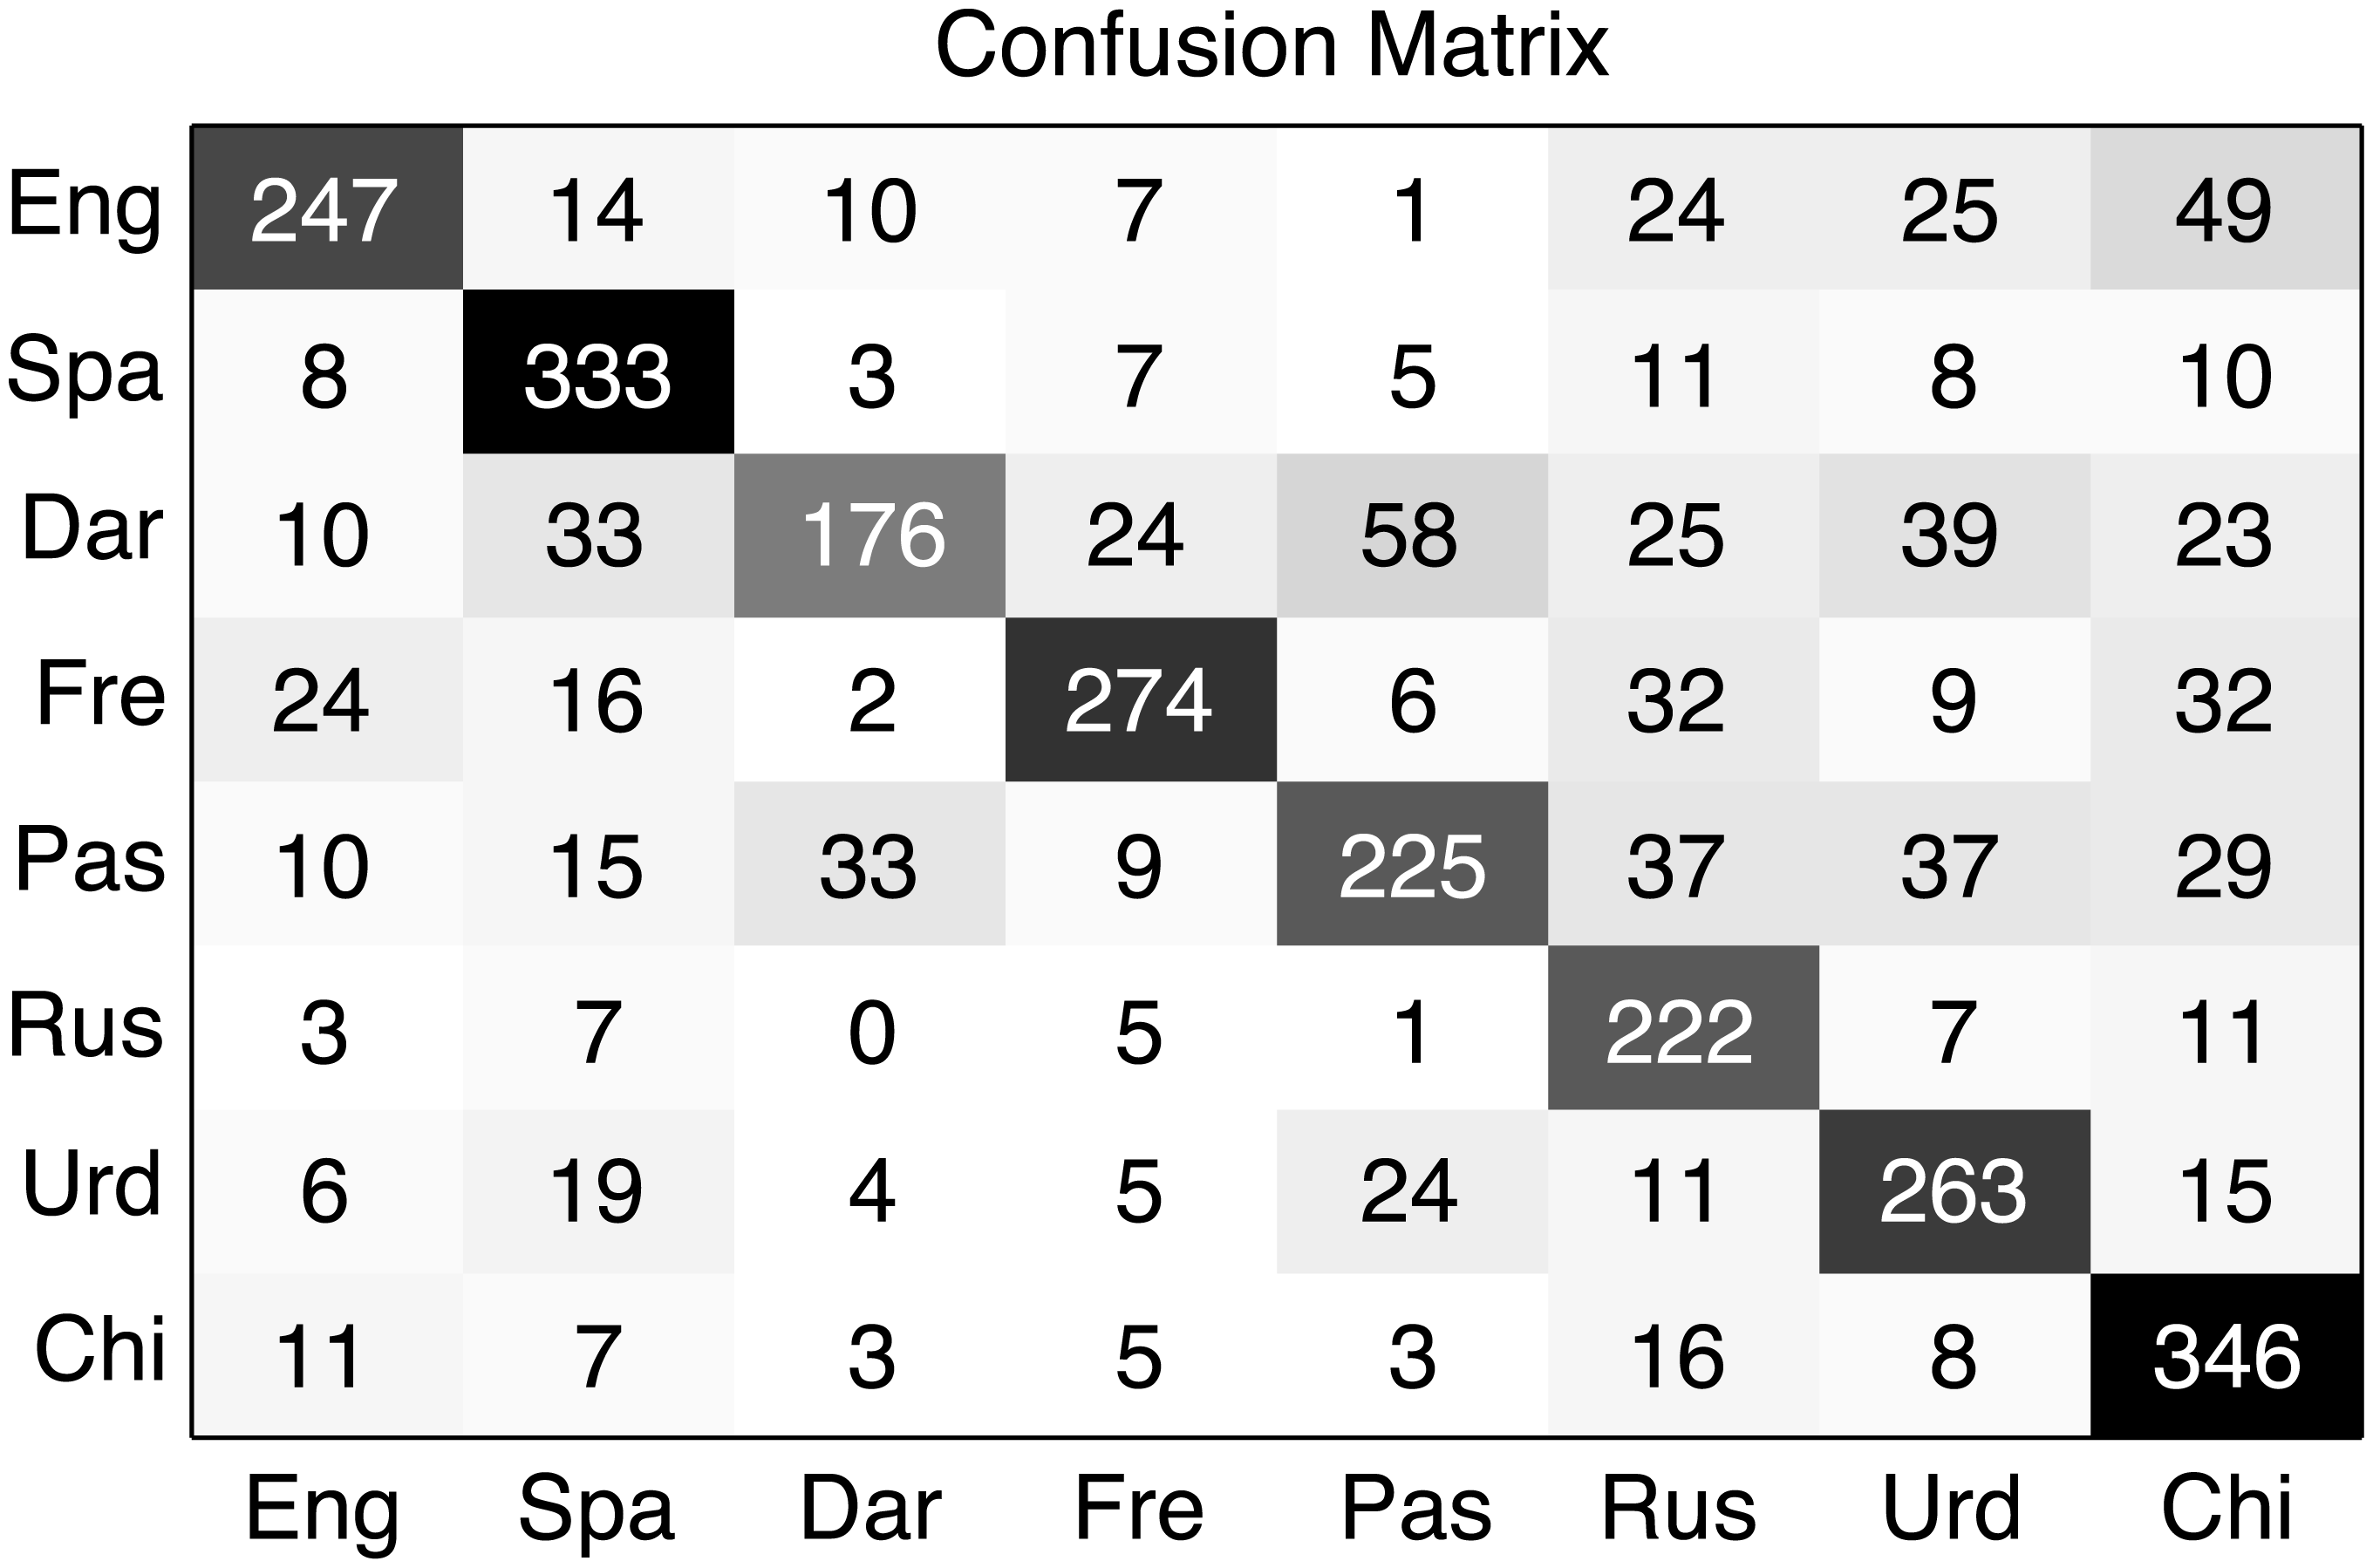
\includegraphics[width=0.6\textwidth, keepaspectratio]{imgs/confusion-matrix.png}
\caption{Example of a confusion matrix.}
\end{figure}
\noindent
The diagonal represents correct detections for that class. The rows and columns represent false positives and false negatives, as they are predicted the wrong class. Confusion matrices are useful to see which classes are better predicted compared to other classes

\subsection{Validation}
Because testing data is sometimes completely hidden, the given training data may need to be split into a validation set, which is used to evaluate the quality of the model. There is an issue during the splitting phase of training and validation data where the two sets are not good representation samples from the dataset. For example, if the dataset is split in half exactly, many important features may be missed. 
\begin{figure}[H]
\centering
\begin{subfigure}{0.4\textwidth}
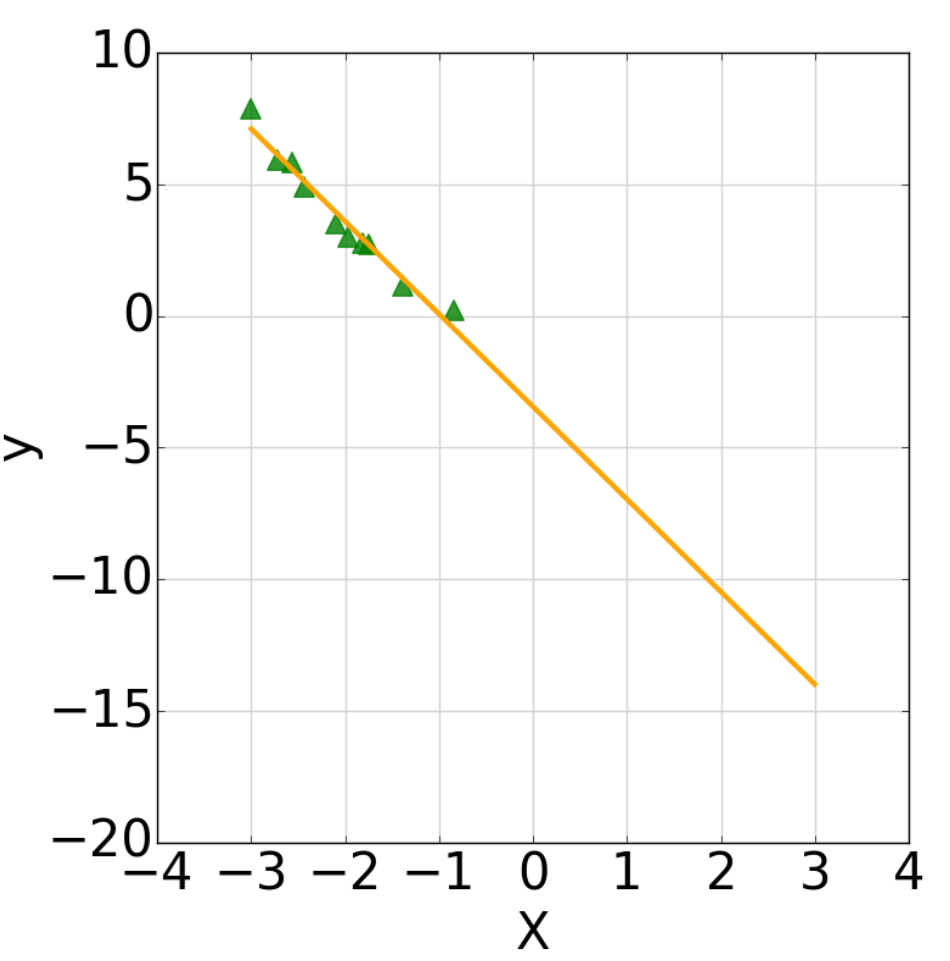
\includegraphics[width=1\textwidth]{imgs/validation-training.png}
\caption{Prediction on training data}
\end{subfigure}
~
\begin{subfigure}{0.4\textwidth}
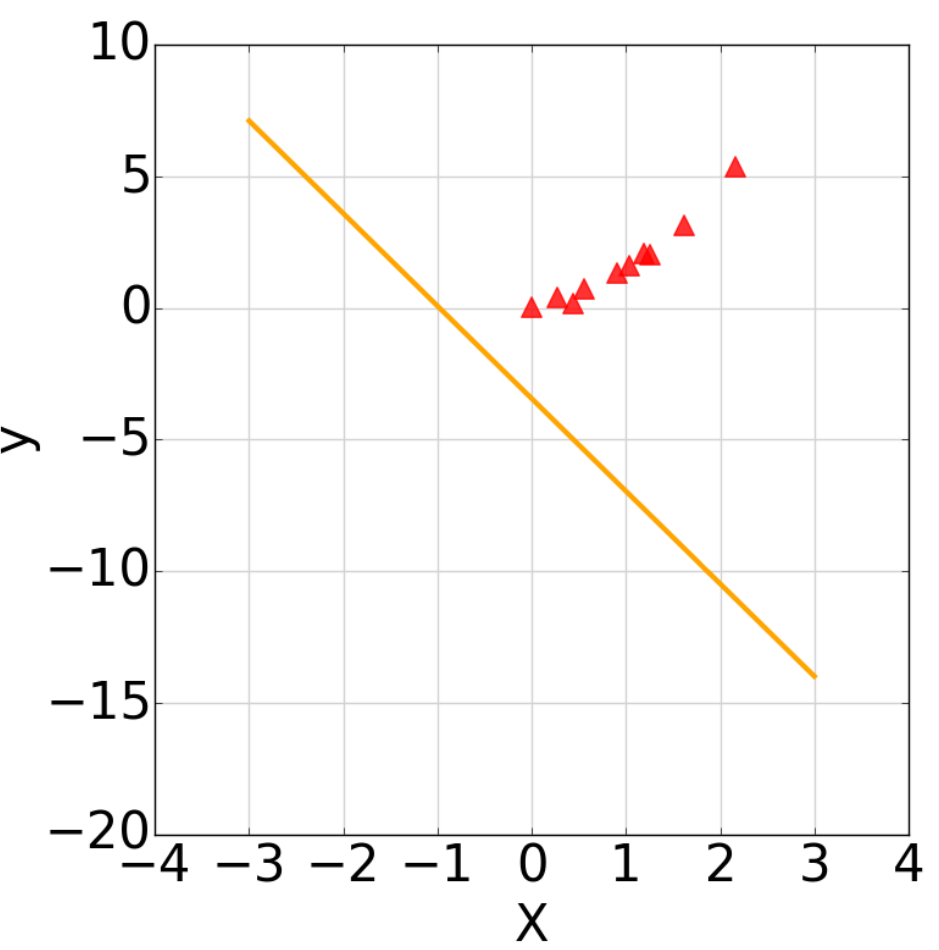
\includegraphics[width=1\textwidth]{imgs/validation-validation.png}
\caption{Prediction on validation data}
\end{subfigure}
\caption{Extreme example of an issue that can occur in splitting training/validation data.}
\end{figure}
\noindent
The split training/validation datasets have to be representative samples from the domain of the entire dataset. However, this can be difficult to do without looking at the dataset, which compromises the experiment. A method to deal with this is called \textbf{stratified sampling}. In classification, this would ensure a representative number of classes are in each dataset. For regression problems, certain important features need to be used as the feature for stratification, for example gender proportions in data about people. 
\n
Another issue with splitting the data into a validation set is that it reduces the amount of data available for training. Further, randomly splitting the dataset, even with stratified sampling could lead to getting ``easier" or ``harder" datasets to work with. Another method to evaluate the performance of trained models is \textbf{k-fold cross validation}.

\subsubsection{k-fold cross validation}
The idea behind k-fold cross validation is to split the dataset into $k$ equally sized subsets and run training $k$ times, leaving out one of the subsets for testing. Each $k$ samples is used for validation exactly once. Larger values of $k$ means more splitting up of the data, which gives more reliable results, but requires more computation.
\begin{figure}[H]
\centering
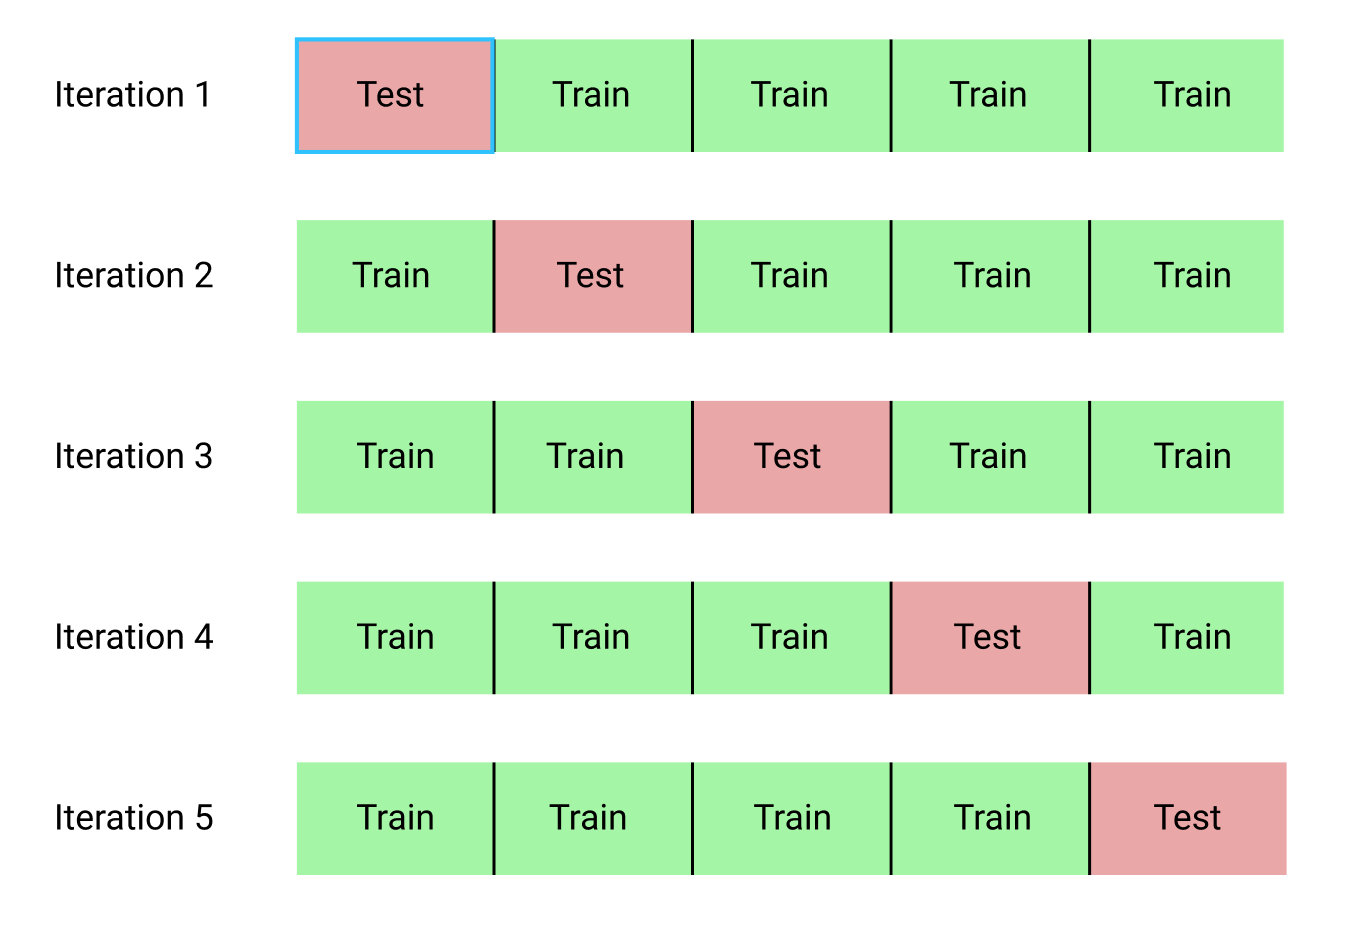
\includegraphics[width=0.7\textwidth, keepaspectratio]{imgs/k-fold-cross-validation.png}
\caption{Example of 5-fold cross validation.}
\end{figure}

\section{Data preparation}
Often times the raw data received at the start of the machine learning process requires cleaning or preprocessing. This can be due to errors during data gathering, for example negative readings that aren't possible, or the way the data is presented, such as categorical values like colour (red, blue, green) or time. Data such as this has to be processed to be able to be passed to any machine learning algorithm, as we need numerical inputs in some cases.
\n
Example data preparation process:
\begin{itemize}
\item Clean data
\item Convert data types (categorical with dummy variables)
\item Find mean and standard deviation of features
\item Normalise data
\item Select a subset of features
\item Split into training and test/validation set
\item Train algorithm
\item Evaluate on test set
\end{itemize}
\subsection{Categorical inputs}
\begin{table}[H]
\centering
\begin{tabular}{| c | c | c | c |}
\hline
\textbf{Make} & \textbf{Horsepower} & \textbf{Color} & \textbf{Accidents} \\
\hline
Aubi TT & 220 & Red & 13 \\
\hline
Citreom C4 & 160 & Blue & 1 \\
\hline
Fauxhall Corso & 98 & Red & 2 \\
\hline
Citreom C4 & 124 & Black & 0 \\
\hline
Aubi TT & 196 & Red & 7  \\
\hline
\end{tabular}
\caption{Example data with categorical inputs (colour)}
\end{table}
Some algorithms such as decision trees and random forests can deal with categorical data, but for models such as linear regression, numerical data is required. There are two main methods of transforming categorical inputs into numeric inputs: \textbf{enumeration} and \textbf{dummy variables}.
\subsubsection{Enumeration}
To encode categories by enumeration, each class of the category can be assigned a number, for example assigning red = 1, blue = 2 etc. This is a very simple way to transform categories to numbers but creates a new issue. The distance between the numbers subtly implies a similarity between the values. For example if red = 1, blue = 2 and black = 3, we are implying that blue is similar to both red and black while red and black are not as similar to each other. Sometimes this can be desirable if encoded correctly to give more detailed information, such as if the colour numbers were ordered in a way that represented the difference. 
\begin{table}[H]
\centering
\begin{tabular}{| c | c | c | c |}
\hline
\textbf{Make} & \textbf{Horsepower} & \textbf{Color} & \textbf{Accidents} \\
\hline
1 & 220 & 1 & 13 \\
\hline
2 & 160 & 2 & 1 \\
\hline
3 & 98 & 1 & 2 \\
\hline
2 & 124 & 3 & 0 \\
\hline
1 & 196 & 1 & 7  \\
\hline
\end{tabular}
\caption{Transformed categorical make and colour data using enumeration}
\end{table}

\subsubsection{Dummy variables}
Instead of enumerating all the categorical values, a vector of ones and zeroes is used where each value corresponds to each possible category and the 1 or 0 represent true and false. 
\begin{table}[H]
\centering
\begin{tabular}{| c | c | c | c | c | c | c | c |}
\hline
\textbf{TT} & \textbf{C4} & \textbf{Corso} & \textbf{Horsepower} & \textbf{Red} & \textbf{Blue} & \textbf{Black} & \textbf{Accidents}\\
\hline
1 & 0 & 0 & 220 & 1 & 0 & 0 & 13 \\
\hline
0 & 1 & 0 & 160 & 0 & 1 & 0 & 1 \\
\hline
0 & 0 & 1 & 98 & 1 & 0 & 0 & 2 \\
\hline
0 & 1 & 0 & 124 & 0 & 0 & 1 & 0 \\
\hline
1 & 0 & 0 & 196 & 1 & 0 & 0 & 7 \\
\hline
\end{tabular}
\caption{Transformed categorical make and colour data using enumeration}
\end{table}

\subsection{Input cleaning}
When data is collected, there are often cases where mistakes or other errors appear and have to be cleaned beforehand. For example, all columns having the same data type and all rows having the same number of columns. Further errors can be dealt with in two ways, either try to fix them, for example inserting an average value to replace a NaN value, or remove the row entirely. The latter case may not be desirable in cases with little data. Other examples include spelling errors, negative values, faulty sensors and infinity values. 

\subsection{Feature selection}
It was mentioned before that a reduced feature set can help reduce overfitting in the case of regularisation. In some cases, some features should be discarded entirely, especially if they are not relevant. There are a few good reasons for selecting only relevant features to use:
\begin{itemize}
\item It can improve accuracy with some models and reduce overfitting
\item It can improve interpret-ability, as it is easier to understand models based on fewer parameters
\item It can make infeasible problems feasible by significantly reducing the computational requirements
\end{itemize}
Feature selection can be done via \textbf{univariate tests} where the correlation between each features and the output is calculated and the good well correlated features are selected. Further, correlation between feature pairs can be calculated, as features that are well correlated to each other may be redundant. 
\n
There are also automatic algorithms for feature selection to select the $k$ best features which give the best performance. Most notable, forward and backward stepwise selection. 
\subsubsection{Stepwise selection}
In stepwise selection, features are either incrementally added or removed until the best number of features is found. In forward stepwise selection, each feature is added incrementally, trained on a new model and evaluated on validation or testing data. The best model is kept and another feature is added. This is repeated until the models no longer improve in performance and the best feature subset is selection.
\n
Backwards stepwise selection works the other way by starting with all input features and removing features which affect the model the least. 

\subsection{Data augmentation}
Data augmentation is a good technique both to increase size of the dataset and help models better generalise to new data. This is especially good for complex and modern classifiers, which may only work in very specific cases without data augmentation and need very large amounts of data. Augmentation can be done by transforming existing data in some way. For example shift, rotate, scale, distort, flip, change contrast in images. Domain knowledge is useful here to know how to augment the data. 
\begin{figure}[H]
\centering
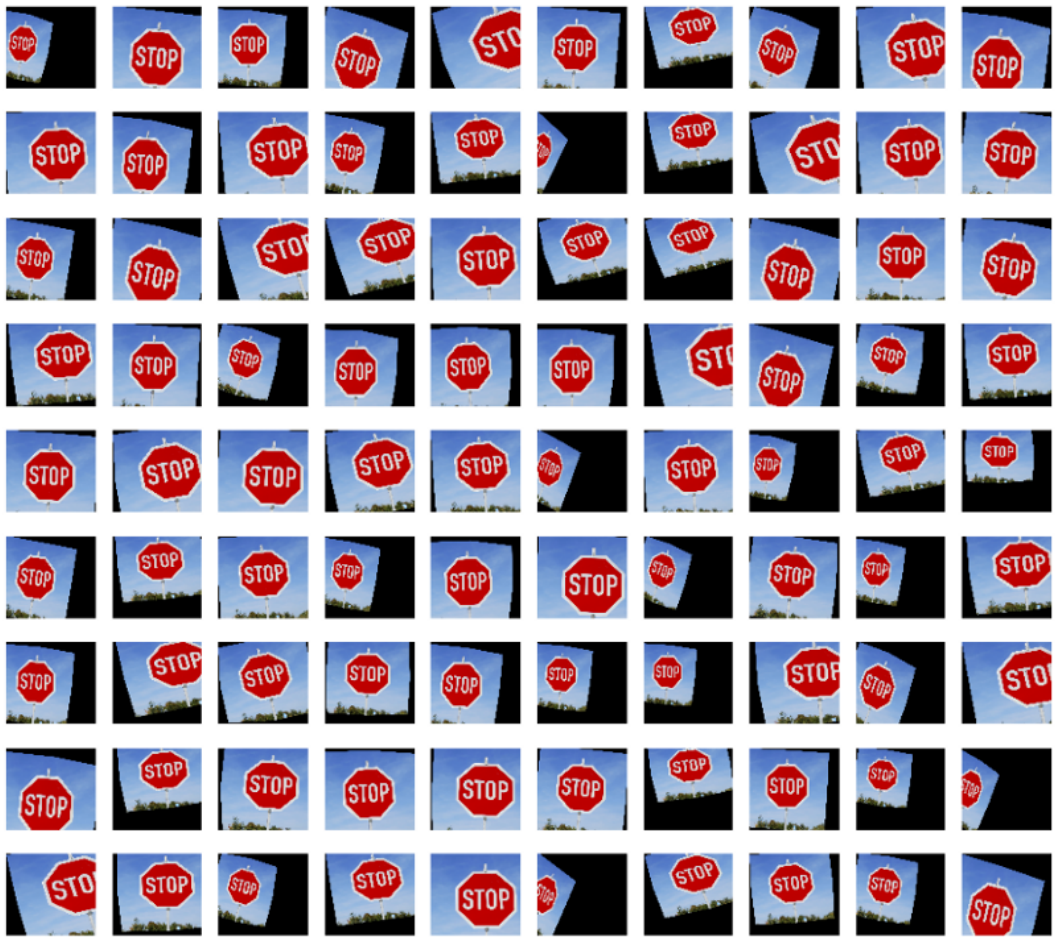
\includegraphics[width=0.6\textwidth, keepaspectratio]{imgs/data-augmentation.png}
\caption{Example of data augmentation on images of a stop sign.}
\end{figure}
 
 
\end{document}